
\documentclass[landscape,a0paper,fontscale=0.34]{baposter} 
\usepackage{comment}
\usepackage{graphicx} 
\graphicspath{{figures/}} 
\usepackage{amsmath} 
\usepackage{amssymb} 
\usepackage{booktabs} 
\usepackage{enumitem} 
\usepackage{palatino} 
\usepackage[font=small,labelfont=bf]{caption} 
\usepackage{multicol} 
\setlength{\columnsep}{1.5em} 
\setlength{\columnseprule}{0mm} 
\usepackage{tikz} 
\usetikzlibrary{shapes,arrows} 

\newcommand{\compresslist}{
  \setlength{\itemsep}{1pt}
  \setlength{\parskip}{0pt}
  \setlength{\parsep}{0pt}}

\newcommand{\bfSigma}{\mbox{\boldmath$\Sigma$}}
\newcommand{\bfLambda}{\mbox{\boldmath$\Lambda$}}
\DeclareMathOperator*{\argmax}{\arg\!\max}
\definecolor{lightblue}{rgb}{0.145,0.6666,1} 

\usepackage{csquotes}
\usepackage[
backend=biber,
style=numeric,
citestyle=numeric
]{biblatex}
\addbibresource{biblio.bib}

\begin{document}

\begin{poster}{
headerborder=closed, 
colspacing=1em, 
bgColorOne=white, 
bgColorTwo=white, 
borderColor=lightblue, 
headerColorOne=black, 
headerColorTwo=lightblue, 
headerFontColor=white, 
boxColorOne=white, 
textborder=roundedleft, 
eyecatcher=true, 
headerheight=0.1\textheight, 
headershape=roundedright, 
headerfont=\Large\bf\textsc, 
linewidth=2pt 
}

%	TITLE SECTION 
{
\includegraphics[height=3em]{milalogo}} % First university/lab logo on the left
{\bf\textsc{Applying LSTM to text classification and generation}\vspace{0.5em}} % Poster title
{\textsc{J. Leroux, N. Laliberte, F. Boileau \hspace{5pt}\hspace{5pt} }} % Author names and institution
{
\includegraphics[height=3em]{udemlogo}} % Second university/lab logo on the right

%	STABILITY SELECTION
\headerbox{Introduction}{name = intro, column = 0, span = 2}{


Recurrent neural networks (RNN) constitute a family of neural network architectures
specialized to process sequential data. They do so by leveraging the simple idea
of sharing parameters across the model\cite{deeplearning}. They have been used in diverse domains for
generating sequences such as music and text. They can be trained by processing
real data sequences one step at a time and predicting what comes next.
In practice, early RNNs designs are unable to store information about far past
inputs. This fact diminishes their efficiency at modeling long structure. If
the network's predictions are based only on the last few inputs, which are
themselves predicted by the networks, then it has less chance to recover from
past mistakes. The solution to this problem seems to be a better memory and
especially a long-term memory for the network. 

\vspace{0.1in}

Long Short-Term Memory (LSTM) are RNN designed to solve this problem. They are
better at storing informations than standard RNNs. It is important to note that
LSTM gives state-of-the-art results in a variety of sequence processing tasks.
This is the main reason why we decided to implement a LSTM for our text
generation project. We worked on 4 differents dataset: Harry Potter's books,
Lord of the ring's books, random quotes and a text from Shakespeare. }

\headerbox{Recurrent Neural Networks}{name = rnn, column = 0, below = intro, span = 2}
{
\begin{multicols}{2}
RNN comes from the following question: is there a neural network that depends
on the full previous context that would model: \begin{align*}
    P(o_1, \dots , o_T) = \prod_{t = 1}^T P(o_t | \hspace{0.05in} o_1, \ldots o_{t-1})
\end{align*}

They are feedforward neural networks with the addition of time dependency in
the model by introducing edges that span the adjacent time steps in the
network. At a given time, the nodes with recurrent edges receive input from the
current data and from the output of the hidden layer in the previous state, see
figure below. Thus, an input at time $t$ can influence the output at time $t + \delta$.
\begin{center}
    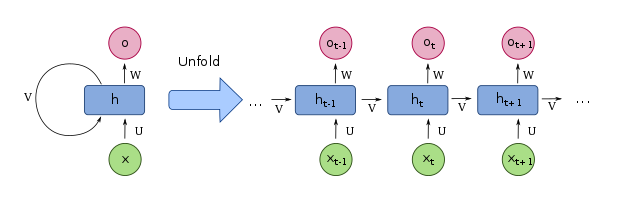
\includegraphics[width = 0.9\linewidth]{RNN.png}
\end{center}

Each time step are computed as follows:
\begin{align*}
    &h_t = \sigma(U x_t + V h_{(t-1)} + b_h)\text{,}\\
    &o_t = \text{softmax}(W h_t + b_o)
\end{align*}

Here, $ U$, $V$ and $W$ are weights matrix. The vectors $b$ are bias
parameters. Learning with RNN is challenging due to dependencies between long
time steps. Consider the gradient with respect to $h_t$ of $o_{t + \delta}$.
How does it vary with $\delta$? Following the graph above and applying the
chain rule we can see that
\begin{equation*}
  \nabla_{h_t} o_{t + \delta} = \left( \prod_{k = t+1}^{t+\delta} V^T
  \text{diag}(1 - h^2_k) \right)\nabla_{h_{t + \delta}}o_{t + \delta}.
\end{equation*}

Thus, as $\delta$ grows, the gradient grows exponentially with $V$. If $V$ is
small or large than the gradient will either vanish or explode. This problem is
well known. Solutions exist, which brings us to present the LSTM.
\end{multicols}
}

\headerbox{Long-Short-Term Memory}{name = lstm, column = 0, below = rnn, above = bottom, span = 2}{

\begin{multicols}{2}
The LSTM model has been introduced primarily to solve the vanishing and
exploding gradients problem. This model is a RNN in which we replaced every
hidden nodes by a \textit{memory cell}.  \begin{center}
    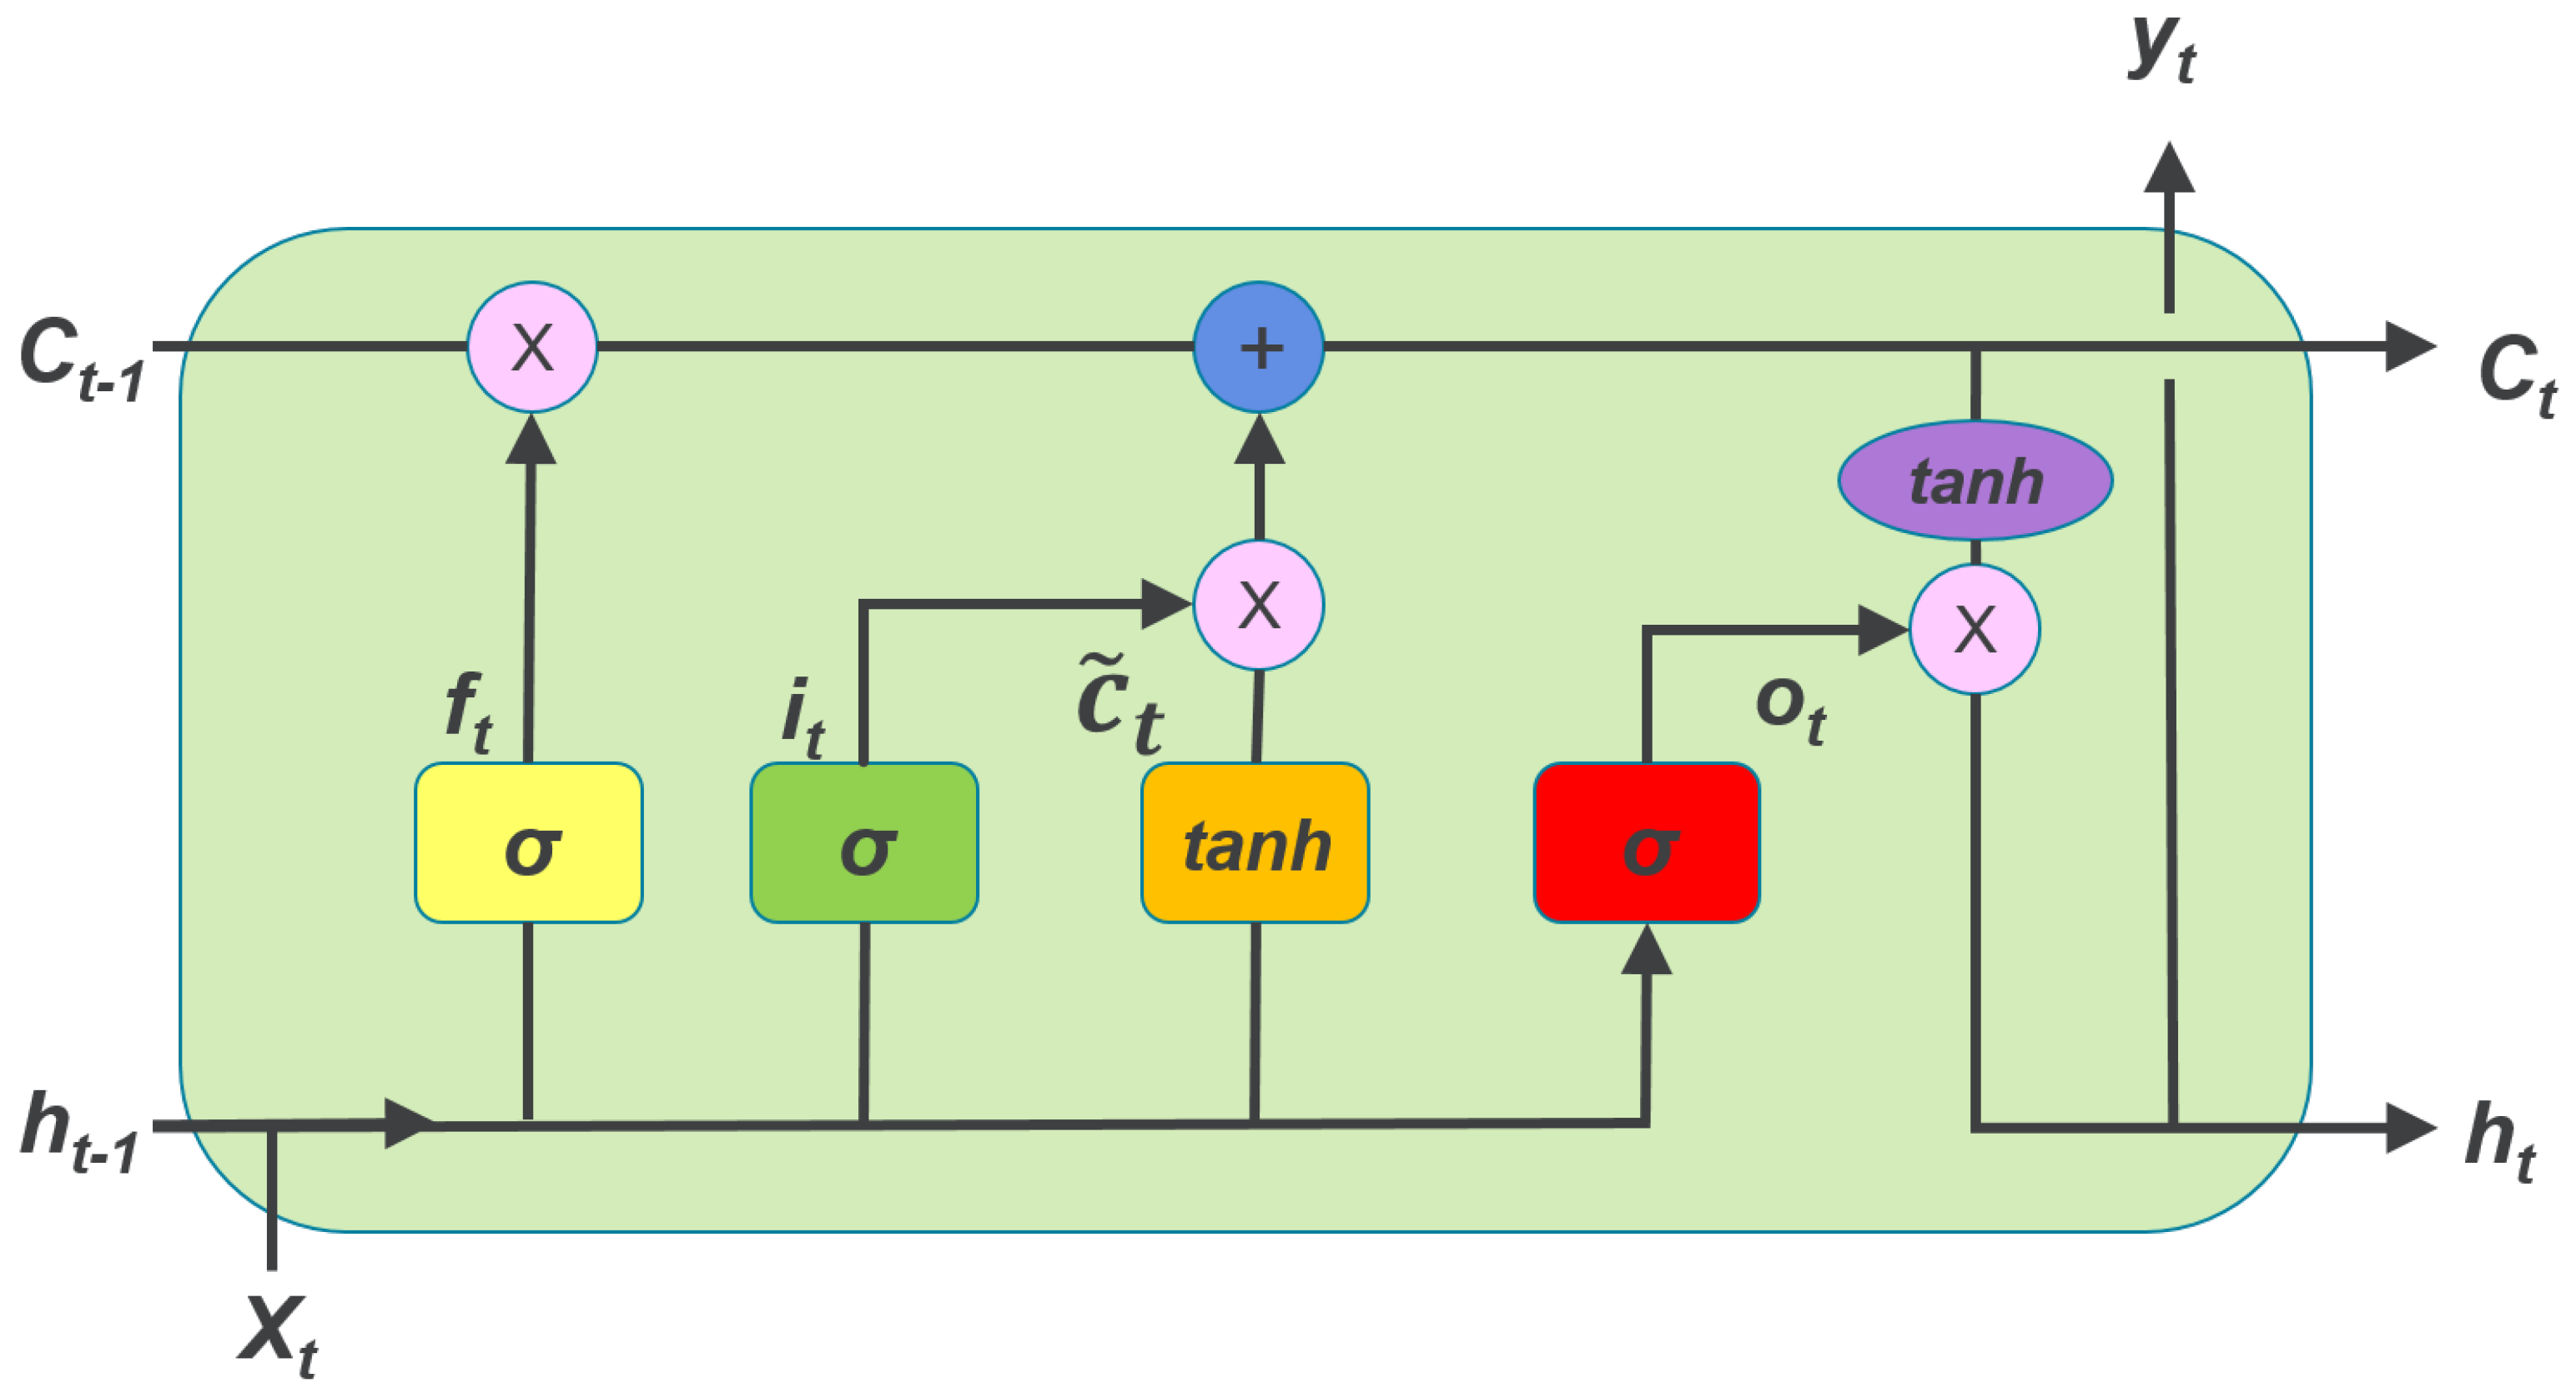
\includegraphics[width = 0.7\linewidth]{lstm.png}
\end{center}

Intuitively, RNN have \textit{long-term memory} in the form of matrix weights,
they change during the training encoding general knowledge about the data. RNN
also have \textit{short-term memory} in the form of activation passing from
each node to successive ones. The memory cell introduced in the LSTM model
provides storage for those memories. We now describe components of the cell
following.\cite{review}

\begin{center}
    \begin{itemize}
    \item Gates ($f_t, i_t, o_t$): They are sigmoidal units that takes
      activation from the input $x_t$ and the output of the hidden layer from
      previous state $h_{t-1}$. Note that $f_t$ multiply the value of the
      previous cell $c_{t-1}$. The term \textit{gate} stands for the literal
      meaning in the sense that if $f_{t}$ is close to $0$, then the gate is
      \textit{closed} and the flow from the previous cell is cut off. If $f_t$
      is closed to $1$ then all flow is passed through. The output to the
      hidden layer is $h_t = o_t \odot \tanh(c_t)$ where $\odot$ denote the
      pointwise multiplication.
    \item Cell state ($c_t = f_t \odot c_{t-1} + i_t \odot \tilde{c}_t$): Cell
    state maintains information on the input. Also refered as the internal state,
    $c_t$ has a self-connected edges with a fixed unit weight. This constant
    weight implies that the error can flow across time without vanishing or
    exploding. 
\end{itemize}
\end{center}
\end{multicols}}

%	SIMULATION STUDY 
\headerbox{Results}{name = results, column = 2 ,span = 2, row = 0}{
\vspace{0.05 cm}

\subsection*{Implementation goal}
\begin{multicols}{2}
For the implementation section of this project, we gathered text data that we
found around the internet to train a sequence classifier and generate text
sequences. The training of the classifier consist of identifying from which
corpus between Harry Potter, Lord of the rings, some random quotes and
Shakespeare, the sequence corresponds to. Further to this, we trained one model
per sequence type for the text generation. Finally, we verified that our
generated sequences were well classified by our classifier. The parameters we
used for the models are shown in the table below. 

\subsection*{Preprocessing and model details}

Before doing any sort or training, we had to do a bit of preprocessing on the
data. First, we tokenized each corpus in sequences of 50 tokens. Then, we
removed every capital letters to standardize the text. We built up a dictionary
of every tokens ($\approx 60k$) in the datasets, this is our input space. Next,
encode each token in a 256 dimensions vector with en embedding layer. We then
feed the encoded vectors to our LSTMs with a hidden/cell state of 512
dimensions. The output dimension is 4 for the classifier and $\approx 60k$ for
the text genetation. 
\end{multicols}

\begin{multicols}{2}
\subsection*{Classification of sequences}
For the training of our classifier, we used the many-to-one architecture like the one below.
\begin{center}
	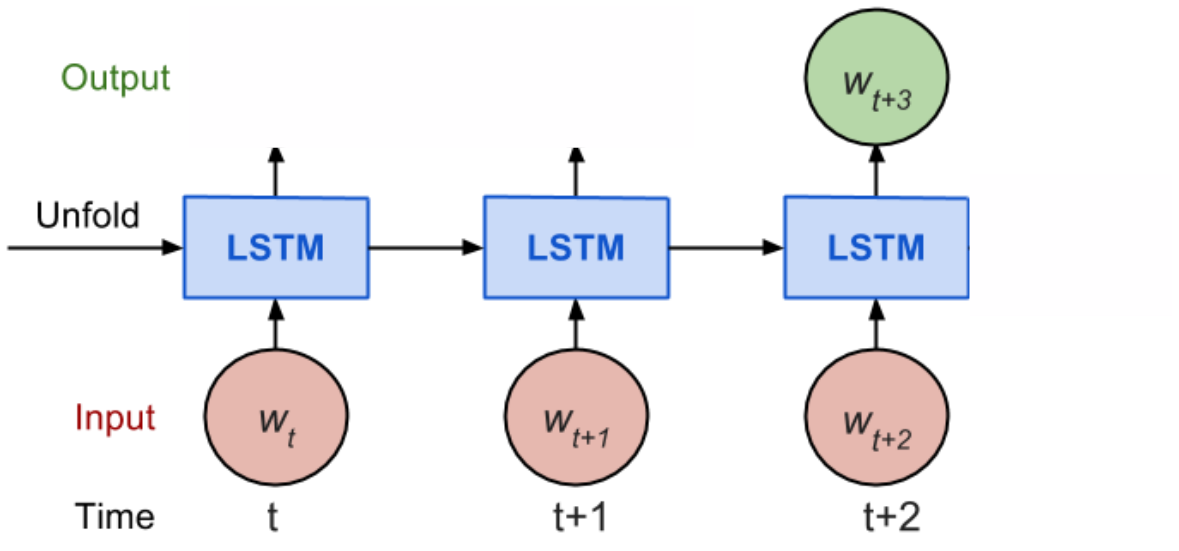
\includegraphics[width=.65\linewidth]{manytoone}
		\captionof{figure}{Many-to-one architecture.}
\end{center}
We used the last output of the LSTM as our input for the classifier,
disregarding all the other outputs. The last hidden state contains information
about about all the sequence through the memory cell.  \begin{center}
	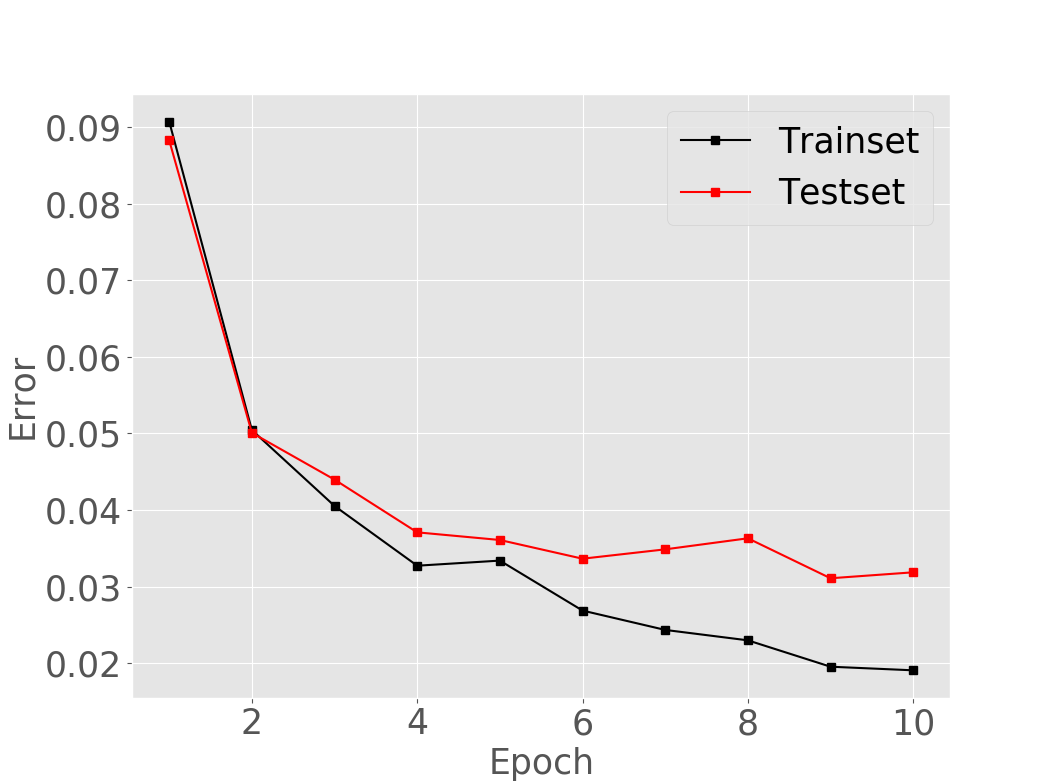
\includegraphics[width=.7\linewidth]{classerror}
	\captionof{figure}{Classification error on train/test set.}
\end{center}
The error we used here is the cross-entropy loss, which is standard for
classification tasks. We see on our training curves (figure 2) that we have
reach 96\% for the classification accuracy.

%------------------------------------------------
\begin{center}
\subsection*{TextGen and Classification}
\end{center}
For the text generation models, we used a many-to-many achitecture like the one
showed in the RNN section. We trained our models by minimizing the
cross-entropy loss. Then, we calculated the average number of extra byte needed
to encode each character. We fixed the average number of character per word to
5. As another standard metric for language modeling, we also calculated the
perplexity of our model \cite{gravesGenerating}. Those results are given in the table below.  \\
\begin{center}
\begin{tabular}{|l|l|c|}
\hline
Dataset & BPC & Perplexity \\
\hline
Harry Potter & 1.00 & 33 \\
LOTR & 1.02 & 35 \\
Random quotes & 1.10 & 45 \\
Shakespeare & 0.94 & 26\\
\hline
\end{tabular}
\end{center}

\begin{itemize}\compresslist
    \item `` well , we ' ll do it with a wand , '' said hermione . `` really ?
      '' said harry , looking at each other .
    \item  what looked about this
      way , the black citadel , was far from the
          darkness , the ring was heard , but the sea big was big , and a great
          ring was in his battle .
    \item failure is a beginning of love and a family which comes from god .
    \item  '' that now my mind shall screens his music , '' '' and i to give
      thee my vulgar heaven , '' '' i am your brother .
\end{itemize}
For the generation of sequences, we initialize our LSTM with a random word
drawn from our dictionary. Next, we feed back the prediction in the network
until we reach the desired sequence length. We generated 1000 sequences (250
per models) and used our classifier on them. A few examples of generated
sequences are shown above. With no surprise, we scored 98\% on the
classification task, which confirms that our sequences are at least probable.

\end{multicols} }

%----------------------------------------------------------------------------------------
%	REFERENCES
%----------------------------------------------------------------------------------------
\headerbox{References}{name=ref, column = 2, span = 2, below = results, above = bottom}{
\printbibliography
}

\begin{comment}
\headerbox{Further Work}{name=conclusion,column=2,span=2,below=CLSA,above=bottom}{
\begin{itemize}\compresslist
\item Exploration and development of loss functions on unknown graph structure is a relevant idea.
\end{itemize}
\vspace{0.3em} }
\end{comment}
\end{poster}
\end{document}
